\section{学习行为与案例：模型是否真的学会把证据放到显著区域}

本章结论是：MemOCR 的收益来自“视觉表示 + 训练后版面策略”的组合；训练过程分析和 case study 共同指向同一个机制，模型在强化学习（reinforcement learning, RL）之后逐渐学会把直接决定答案的证据放入 \textit{crucial area}，把 supporting facts 和 detail descriptions 放入 \textit{detail area}。换句话说，layout control 在这里承担了三重角色：记忆索引、重要性标注、压缩率分配器。

\subsection{训练过程中 evidence placement 的变化}

上一章的 oracle analysis 已经说明，正确答案或关键证据放在 \textit{crucial area} 时，在低 memory budget 下带来的收益最大；放在 detail area 时，收益较弱，某些高压缩设定还会因为可读性下降而拖累表现。讲者随后追问了一个更关键的问题：这种效果是否真的被模型学到了，还是只在人工注入 oracle evidence 时成立？

回答来自训练 step 分析。实验统计模型在不同训练阶段把正确答案相关证据放入 \textit{crucial area} 和 \textit{detail area} 的比例。随着训练推进，关键证据进入 crucial area 的比例明显上升；相应地，同类证据进入低显著区域的比例下降。这说明模型逐步形成了可观察的 evidence placement 行为，而非随机把信息写到画布上。

\begin{figure}[H]
\centering
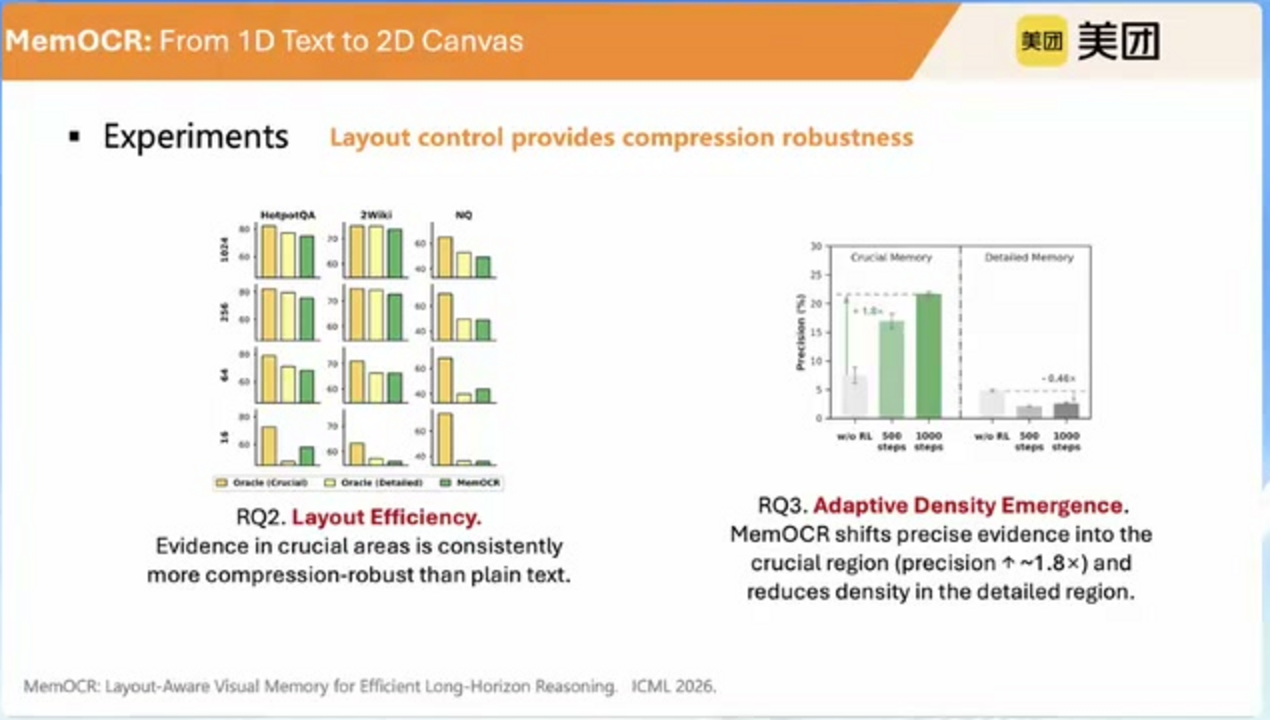
\includegraphics[width=0.84\linewidth,height=0.36\textheight,keepaspectratio]{figures/selected/fig06_layout_efficiency_density.png}
\caption{Layout efficiency 与 adaptive density emergence：左侧复核 oracle 注入位置对压缩鲁棒性的影响，右侧显示训练推进后关键证据更常进入 crucial area，detail area 的密度相应下降。\protect\footnotemark}
\label{fig:layout-efficiency-density}
\end{figure}
\footnotetext{视频画面时间区间：00:15:30--00:16:00。若为裁剪图，时间区间仍对应原视频画面。}

图 \ref{fig:layout-efficiency-density} 的读法很直接：左侧回答“关键证据放在哪里更抗压缩”，右侧回答“模型训练后会不会主动这样放”。右侧图中的 \textit{precision} 上升不是一个抽象审美指标，它对应的是关键证据落在可读区域的概率。对长程推理来说，这相当于把旅行箱里最重要的证件放在最容易拿到的夹层，而把衣物和备用物品放进更深的位置；容量紧张时，先被保住的应当是会改变最终答案的东西。

\begin{importantbox}{机制判断}
MemOCR 的学习目标包含两件事：模型要会读压缩图，也要会写经得起压缩的图。当正确答案相关证据进入 high-level headings、粗体块、靠前区域或更醒目的版面单元时，下采样和 image token 限制带来的损失会先落在辅助细节上，关键证据更容易存活。
\end{importantbox}

为了把这个行为说得更精确，可以用一个讲义抽象来描述一条信息的版面位置：

$$
L(I_i) = (x_i, y_i, s_i, \rho_i)
$$

其中：

\begin{itemize}
  \item $L$：layout function，表示把信息放到画布上的规则。
  \item $I_i$：第 $i$ 条待写入记忆的信息。
  \item $(x_i,y_i)$：这条信息在二维画布上的位置。
  \item $s_i$：视觉显著性，例如标题层级、字号、颜色、空白边界或靠近中心的位置。
  \item $\rho_i$：压缩配置或信息密度，例如字号、行距、局部文字密度，以及下采样后仍能被读出的概率。
\end{itemize}

这个公式属于讲义抽象，用来把讲者的机制压缩成可操作的设计语言；它不代表论文原始公式。若 $I_i$ 是 final answer 的关键证据，理想策略会提高 $s_i$，降低局部压缩压力；若 $I_i$ 只是 supporting fact，则可以承受更高的信息密度。

\subsection{Case study：16-token budget 下证据如何存活}

训练曲线给出总体趋势，case study 则展示这个趋势在单个问题上如何改变答案。图 \ref{fig:case-study-layout-control} 的问题是：\textit{Who wrote ``Put Your Hand in the Hand'' of the man who stilled the water?} 正确答案是 \textit{Gene MacLellan}。这个例子有两个关键实体：\textit{Ocean Band} 和 \textit{Gene MacLellan}。如果这两个实体中的任何一个在压缩过程中消失，后续推理链就会断裂。

\begin{figure}[H]
\centering
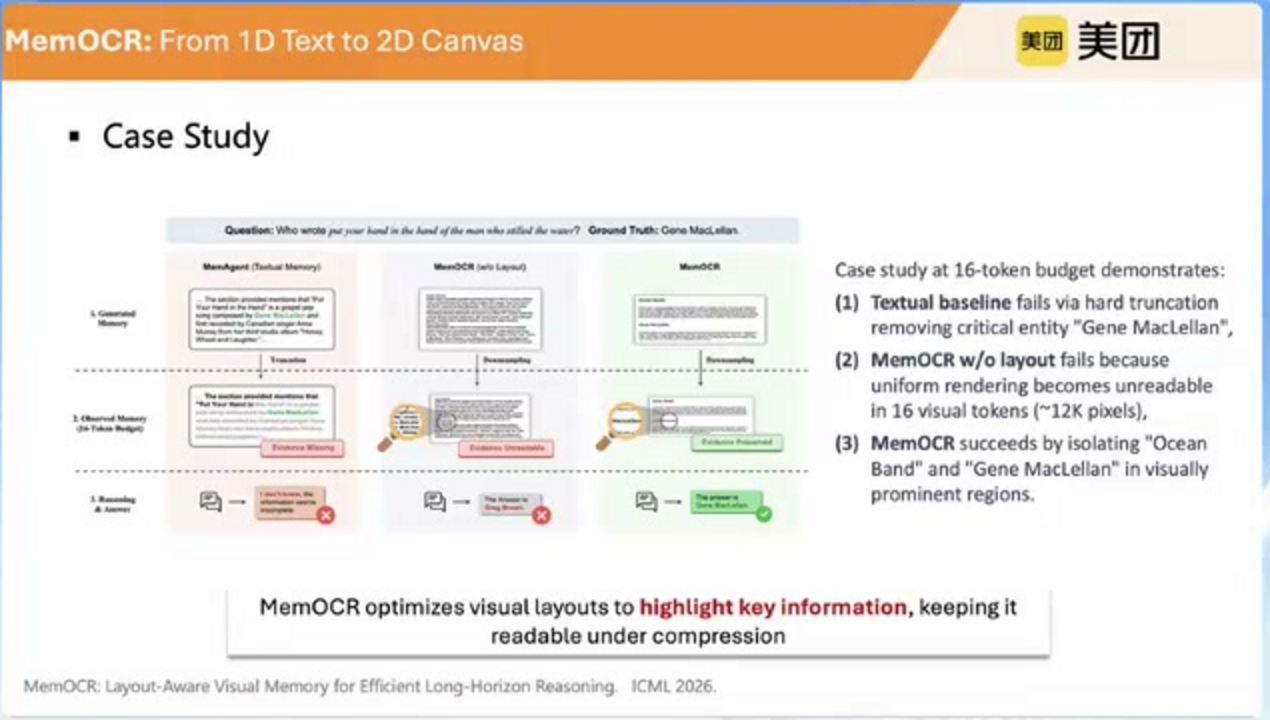
\includegraphics[width=0.86\linewidth,height=0.40\textheight,keepaspectratio]{figures/selected/fig07_case_study_layout_control.png}
\caption{16-token budget 下的三路对比：文本截断丢失关键实体，无 layout control 的视觉记忆在统一渲染后不可读，MemOCR 通过显著区域保留 \textit{Ocean Band} 与 \textit{Gene MacLellan}。\protect\footnotemark}
\label{fig:case-study-layout-control}
\end{figure}
\footnotetext{视频画面时间区间：00:16:30--00:17:00。若为裁剪图，时间区间仍对应原视频画面。}

这个案例把三种记忆策略的失败和成功拆开了：

\begin{itemize}
  \item \textbf{文本记忆截断}：simple truncation 直接移除了关键实体，回答模型只能面对不完整上下文。
  \item \textbf{无分区视觉记忆}：所有信息以接近均匀的字号和密度写入，16 个视觉记忆 token 下文字变成难以识别的小块，证据仍在图上，但模型读不到。
  \item \textbf{MemOCR}：关键实体被隔离到视觉显著区域，压缩后仍保留可读性，最终回答得以落到 \textit{Gene MacLellan}。
\end{itemize}

这里的关键差异是“证据存在”和“证据可读”之间的差异。文本截断的问题是证据不存在；无布局视觉记忆的问题是证据名义上还在，实际已经不可读。MemOCR 想解决的是第二类更隐蔽的问题：压缩后的表征需要让底层视觉语言模型继续分辨出会影响答案的实体和关系。

\begin{warningbox}{容易误解的地方}
16-token budget 指最终回答阶段用很少的 image tokens 表示视觉记忆；它不能被理解成原图只剩 16 个普通文本 token。读者需要把 memory budget 和 context budget 区分开：前者是记忆表征占用多少预算，后者是模型一次推理能接收的整体上下文容量。
\end{warningbox}

\subsection{为什么显著区域像一个可读索引}

显著区域的作用可以类比一本书的目录和加粗标题。目录不包含所有内容，却告诉读者从哪里进入；加粗标题不替代正文，却在快速扫描时保护核心线索。MemOCR 的 crucial area 也承担这个功能：它把答案相关证据放到更容易被压缩后识别的位置，让模型在有限 image tokens 下先读到“该往哪儿想”。

这解释了为什么 oracle injection 放进低效区域可能损害性能。低显著区域本来就承担更高压缩，继续把答案塞进去会增加局部密度，读者看到的是一页更挤的便签；视觉模型看到的是更难解码的小字块。信息价值和版面密度错配时，加入更多内容会降低可读性。

\begin{knowledgebox}{从训练行为到工程启示}
如果未来把 MemOCR 这类机制用于真实 agent memory，系统需要同时问四个问题：哪些证据最影响 final answer，应该放在画布哪里，能承受多强下采样，压缩后底层模型是否仍能读出实体、数字和关系。只讨论“存了多少信息”会漏掉最危险的一环：存下来的信息可能已经不可读。
\end{knowledgebox}

讲者还补充了主结果表的统计检验：各数据集和 average 上的提升在统计上较为鲁棒。这个补充把 case study 从单例解释拉回总体证据：单个例子说明机制如何发生，训练 step 和统计检验说明这种机制并非孤立偶然现象。

\subsection{本章小结}

本章的核心 takeaway 是：MemOCR 真正学到的是一种 \textit{evidence placement policy}。训练推进后，模型更倾向于把答案相关证据放进 crucial area，并减少这些证据进入 detail area 的比例。case study 进一步说明，在 16-token budget 这种极端压缩下，文本截断会丢证据，均匀视觉渲染会让证据不可读，layout control 则通过显著区域保住关键实体。第 6 章将继续追问一个现实问题：这种视觉记忆策略带来的额外计算成本是否值得。
